%----------------------------------------------------------------------------------------
%	PACKAGES AND OTHER DOCUMENT CONFIGURATIONS
%---------------------------------------------------------------------------------------

% if you're here it means you were interested enough in me try and find our a little more. Why don't you skip the digging and go right to the source?


\documentclass[
	10pt, % Default font size, can be between 8pt and 12pt
]{FreemanCV}


% Handle images:
\graphicspath{{./images/}}


\columnratio{0.40, 0.60} % Widths of the two columns, specified here as a ratio summing to 1 to correspond to percentages; adjust as needed for your content 

% Headers and footers can be added with the following commands: \lhead{}, \rhead{}, \lfoot{} and \rfoot{}
% Example right footer:
%\rfoot{\textcolor{headings}{\sffamily Last update: \today. Typeset with Xe\LaTeX}}

%----------------------------------------------------------------------------------------

\begin{document}

\begin{paracol}{2} % Begin two-column mode

%----------------------------------------------------------------------------------------
%	YOUR NAME AND CURRICULUM VITAE TITLE
%----------------------------------------------------------------------------------------

\parbox[][0.05\textheight][c]{\linewidth}{ % Box to hold your name and CV title; change the fixed height as needed to match the colored box to the right
	\centering % Horizontally center text
	
	{\sffamily\Huge Josh \textbf{Booth}} % Your name
	
	\medskip % Vertical whitespace
	
	%{\cursivefont\Huge\textcolor{headings}{Big Bad Baller}}
	
	\vfill % Push content to the top of the box
}

%----------------------------------------------------------------------------------------
%	WORK EXPERIENCE
%----------------------------------------------------------------------------------------
\vspace*{-4pt}
\section{Work Experience}

% Each job is added with a \jobentry command. Below is an empty one to use as a template:

%\jobentry
%	{} % Duration
%	{} % FT/PT (full time or part time)
%	{} % Employer
%	{} % Job title
%	{} % Description

% All 5 parameters must be supplied but any can be empty if you don't need them

%------------------------------------------------

\jobentry
	{Current, from Jun 2022} % Duration
	{FT} % FT/PT (full time or part time)
	{Microchip Technology} % Employer
	{Applications/Marketing Engineer} % Job title
	{ % Description
	\vspace{-15pt}
	\begin{itemize}[leftmargin=0pt]
		\item Developed various demos on PIC and AVR microcontrollers.
		\item Wrote production-quality embedded C code for customers to use as reference.
		\item Developed microcontroller libraries for abstracted use.
		\item Created PCBs and structural enclosures for the demos.
		\item Led an analytics initiative that produced to better data-driven decisions about our marketing campaign strategies.
	\end{itemize}
	} 

%------------------------------------------------

\jobentry
	{Jun 2017 - Jan 2022} % Duration
	{FT/PT} % FT/PT (full time or part time)
	{United States Naval Research Laboratory} % Employer
	{Electrical Engineer Student Trainee} % Job title
	{ % Description
	\vspace{-15pt}
	\begin{itemize}[leftmargin=0pt]
		\item Used python for various machine learning and data analytic projects such as:
		\item Detecting and classifying objects in satellite imagery.
		\item Recovering RF communications lost to noise (BRNN w/ GRU cells.)
		\item Identifying promotor sequences in DNA to speed-up genome sequence identification (BRNN w/ LSTM cells.)
	\end{itemize}
	} 

%------------------------------------------------

\jobentry
	{Sep 2016, Jun 2022} % Duration
	{FT/PT} % FT/PT (full time or part time)
	{Booth Oil and Gas LLC.} % Employer
	{Prototype Engineer} % Job title
	{ % Description
	\vspace{-15pt}
	\begin{itemize}[leftmargin=0pt]
		\item Designed and manufactured prototypes for novel business problems (see 3D PEEK Printer, AI-Driven Security System).
		\item Offered technical expertise for project planning, cost estimation, and feasibility studies.
		\item I communicated with the client to manage their expectations and incorporate or remove features as their needs changed.
	\end{itemize}
	}
	
% %----------------------------------------------------------------------------------------
% % EDUCATION
% \section{Education} 
% %----------------------------------------------------------------------------------------



% % Each qualification entry is added with a \qualificationentry command. Below is an empty one to use as a template:
% %------------------------------------------------

% \begin{supertabular}{r l} % Start a table with two columns, the table will ensure everything is aligned

% 	%------------------------------------------------
	
% 	\qualificationentry
% 		{2018-2022} % Duration 
% 		{Computer Engineering} % Degree
% 		{Summa Cum Laude; 3.98 GPA; Comp Org SI} % Honors, achievements or distinctions (e.g. first class honors)
% 		{Bachelors of Science} % Department
% 		{Shippensburg University of Pennsylvania} % Institution
	
% 	%------------------------------------------------
	
% 	\qualificationentry
% 		{2018-2022} % Duration
% 		{Mathematics} % Degree
% 		{} % Honors, achievements or distinctions (e.g. first class honors)
% 		{Minor} % Department
% 		{Shippensburg University of Pennsylvania} % Institution
	
% 	%------------------------------------------------
	

% 	%------------------------------------------------

% \end{supertabular}
% % END EDUCATION

%----------------------------------------------------------------------------------------
%	PUBLICATIONS
%----------------------------------------------------------------------------------------

\section{Publications}

%------------------------------------------------

\begin{supertabular}{p{0.05\linewidth} p{0.88\linewidth}} % Start a table with two columns, the table will ensure everything is aligned
	
	%------------------------------------------------
	2023 & \href{
	https://ww1.microchip.com/downloads/aemDocuments/documents/MCU08/ApplicationNotes/ApplicationNotes/AN4889-Using-CIPs-To-Implement-Peltier-Plate-DS00004889.pdf
	}{
	App. Note 4889: Using Core Independent Peripherals (CIPs) to Implement a Peltier Cooled Metal Plate
	\scriptsize\faLink} \\[5pt]
	%------------------------------------------------
	2023 & \href{
	https://www.embedded.com/reducing-bom-cost-in-embedded-systems-using-advanced-mcu-peripherals/
	}{
	Embedded.com - Reducing BOM cost in embedded systems using advanced MCU peripherals
	\scriptsize\faLink} \\[5pt]
	%------------------------------------------------
	% 2023 & \href{
	% 	https://gateway.on24.com/wcc/eh/3685667/lp/4156150/learn-the-smart-way-to-use-on-chip-hardware-accessories-to-replace-discrete-components
	% }{
	% Webinar - Learn the Smart Way to Use On-Chip Hardware Accessories to Replace Discrete Components 
	% \scriptsize\faLink} \\
	%------------------------------------------------
	2018 & \href{
	http://joshbooth.us/wp-content/uploads/2023/08/Machine-Learning-in-Radio-Frequency-Communications.pdf
	}{
	Machine Learning in Radio Frequency Communications
	\scriptsize\faLink} \\[5pt]
	%------------------------------------------------
	2017 & \href{
	http://joshbooth.us/wp-content/uploads/2023/08/poster_SBME_promoter_predictions.pdf
	}{
	Prediction of Bacterial Promoter Sequences using Machine Learning
	\scriptsize\faLink} \\[5pt]
	%------------------------------------------------
	
\end{supertabular}

\medskip % Extra whitespace before the next section

%----------------------------------------------------------------------------------------
%----------------------------------------------------------------------------------------
%----------------------------------------------------------------------------------------

% END OF COLUMN 1

%----------------------------------------------------------------------------------------
%----------------------------------------------------------------------------------------
%----------------------------------------------------------------------------------------


\switchcolumn % Switch to the second (right) column

%----------------------------------------------------------------------------------------
%	COLORED CONTACT DETAILS BOX
%----------------------------------------------------------------------------------------

\parbox[top][0.1\textheight][c]{\linewidth}{ % Box to hold the colored box; change the fixed height as needed to match the box to the left
	\colorbox{shade}{ % Create colored box and specify background color
		\begin{supertabular}{@{\hspace{3pt}} p{0.05\linewidth} | p{0.775\linewidth}} % Start a table with two columns, the table will ensure everything is aligned
			\raisebox{-1pt}{\faPhone} & (717) 494-6466 \\ % Phone number
			\raisebox{-1pt}{\small\faEnvelope} & \href{mailto:boothjmail@gmail.com}{boothjmail@gmail.com} \\ % Email address
			%\raisebox{-1pt}{\small\faLink} & \href{https://joshbooth.us}{joshbooth.us} \\ % Website
			\raisebox{-1pt}{\faHome} & Chandler, AZ \\ % Address
			%\raisebox{-1pt}{\faGithub} & \href{https://github.com/username}{https://github.com/username} \\ % GitHub profile
			%\raisebox{-1pt}{\faLinkedinSquare} & \href{https://www.linkedin.com/in/username}{https://www.linkedin.com/in/username} \\ % LinkedIn profile
			% See fontawesome.pdf in the Fonts folder for all icons you can use
		\end{supertabular}
	}
	\vfill % Push content to the top of the box
}


%----------------------------------------------------------------------------------------
%	ENGINEERING PROJECTS
%----------------------------------------------------------------------------------------

\vspace*{-20pt}
\section{Notable Projects}

% Entry 0 - image on right
% DMX Light Show
\setlength\intextsep{7pt} % image in relation to subsection title
\begin{wrapfigure}[10]{rt}{25pt} % # of narrow lines, right top alignment, image L/R adjustment
	\hspace*{-23pt} % how close horizontal text can be
    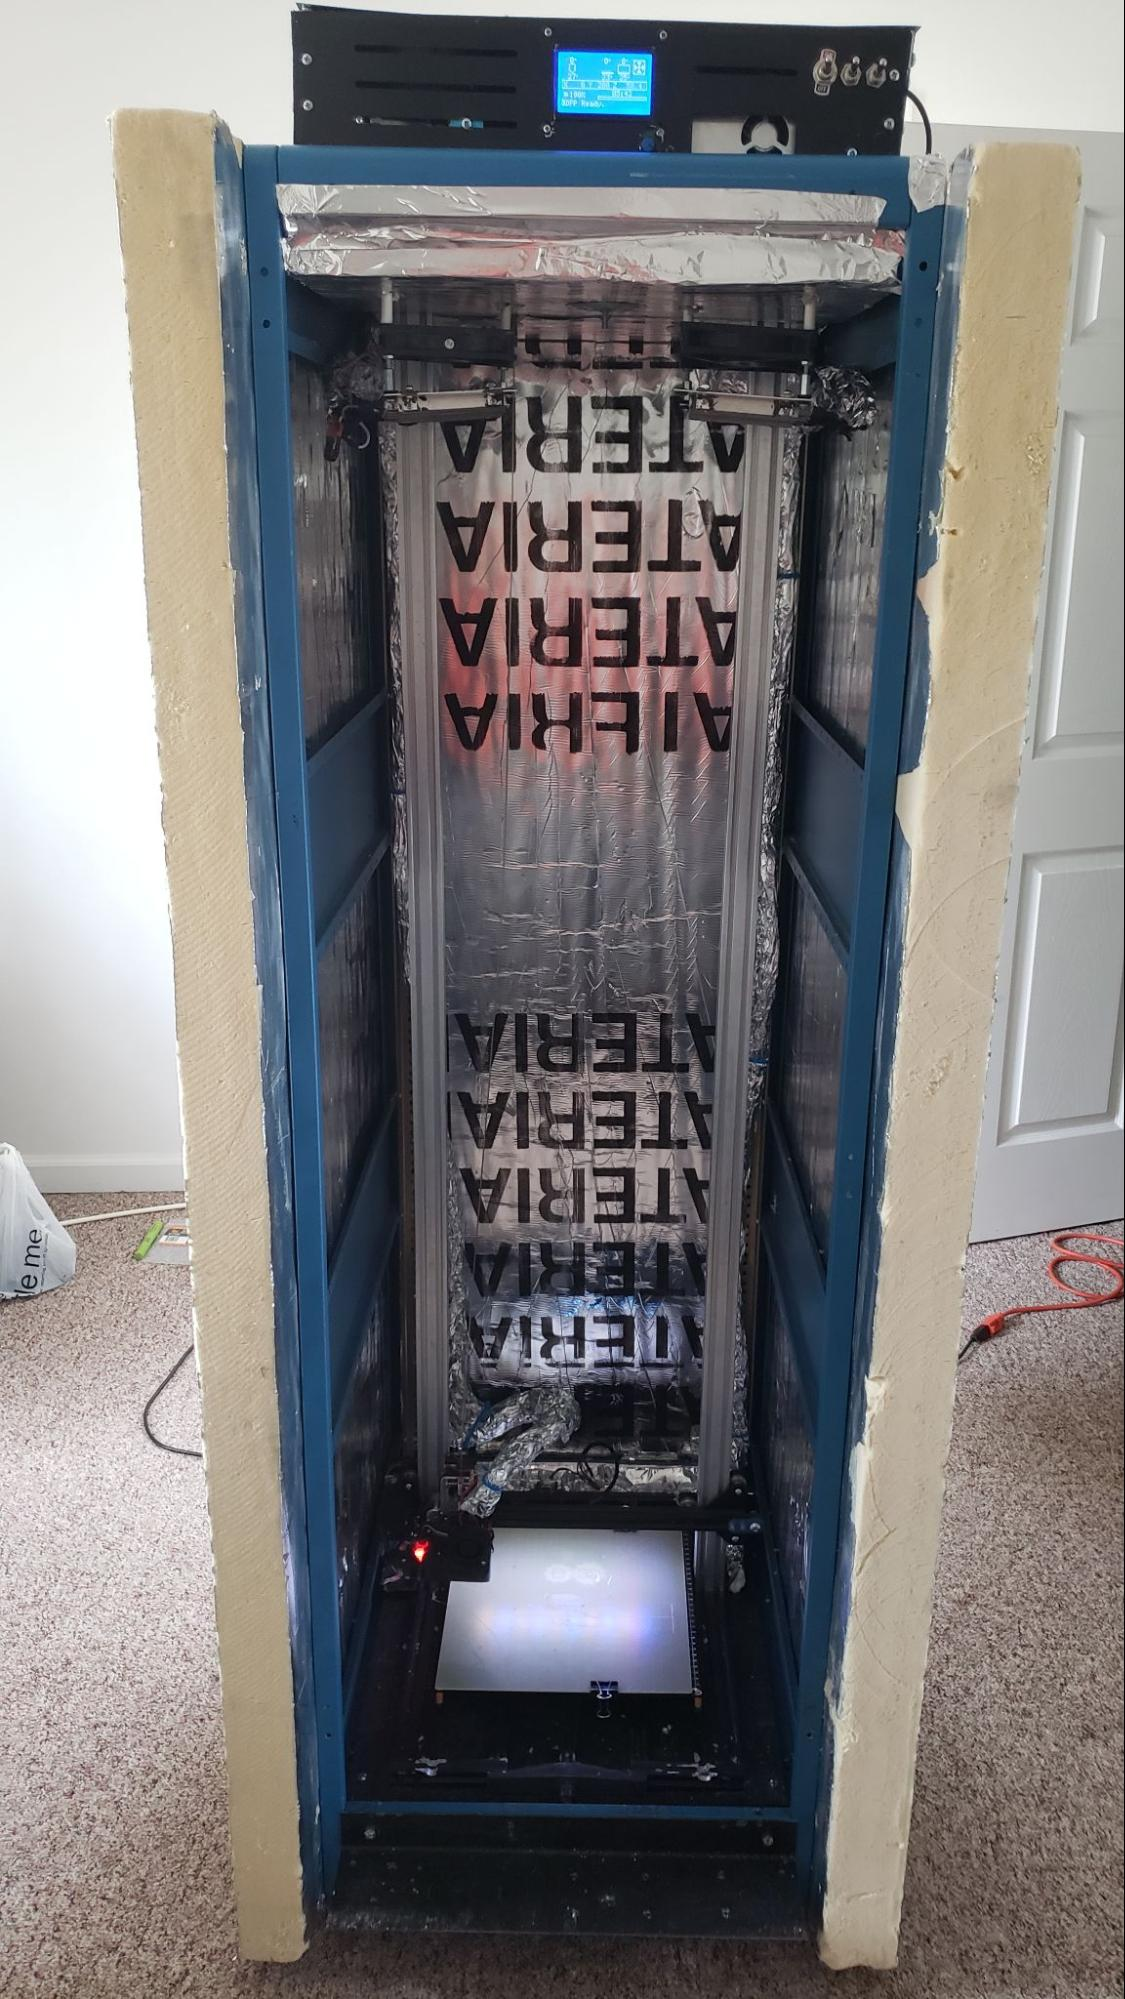
\includegraphics[width=75pt]{printer} %Z how large image is
\end{wrapfigure}

\vspace*{-10pt} % move title's anchor box up closer to title
\leavevmode\subsection{\href{https://github.com/jfcbooth/3dpp}{DMX Light Show \scriptsize\faLink}}

A real-time audio processing light show highlighting the flagship features of the PIC18Q71 microcontroller.
The design extracts bands of audio frequencies (bass, mid, treble, etc.) and sends the lighting information over DMX to 1 of 7 nodes to create a audio-esponsive light show.
Some of the project's technical hurdles involved the design for proper low-noise analog and power design on the same PCB, fault-tolerant DMX and SPI communications, and implementing PoE for the high power requirements.


% Entry 1 - image on left
% AI Driven Security system

\setlength\intextsep{20pt} % how far image is down from section title
\begin{wrapfigure}[7]{l}{30pt} % # of narrow lines, right top alignment, image L/R adjustment
	%\hspace*{-20pt} % how close horizontal text can be
    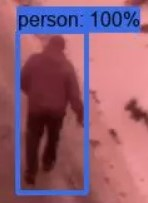
\includegraphics[width=50pt]{security_system} %Z how large image is
\end{wrapfigure}

\vspace*{-10pt}
\leavevmode \subsection{\href{https://github.com/jfcbooth/security_system}{AI-Driven Security System \scriptsize\faLink}}
%\vspace*{-5pt} % move image's anchor box up closer to title

Protoype engineer for a solar-powered security system that gives real-time alerts with a classified video anytime a human, vehicle, or large animal is spotted
on the property. The client also wanted all footage to be stored locally for legal purposes, so a custom program extracted motion clips
after the footage was saved, which could then be reliably transported back to a central node to do the ML classification on.

% Entry 2 - image on right
% 3D PEEK Printer

\setlength\intextsep{7pt} % image in relation to subsection title
\begin{wrapfigure}[8]{rt}{25pt} % # of narrow lines, right top alignment, image L/R adjustment
	\hspace*{-23pt} % how close horizontal text can be
    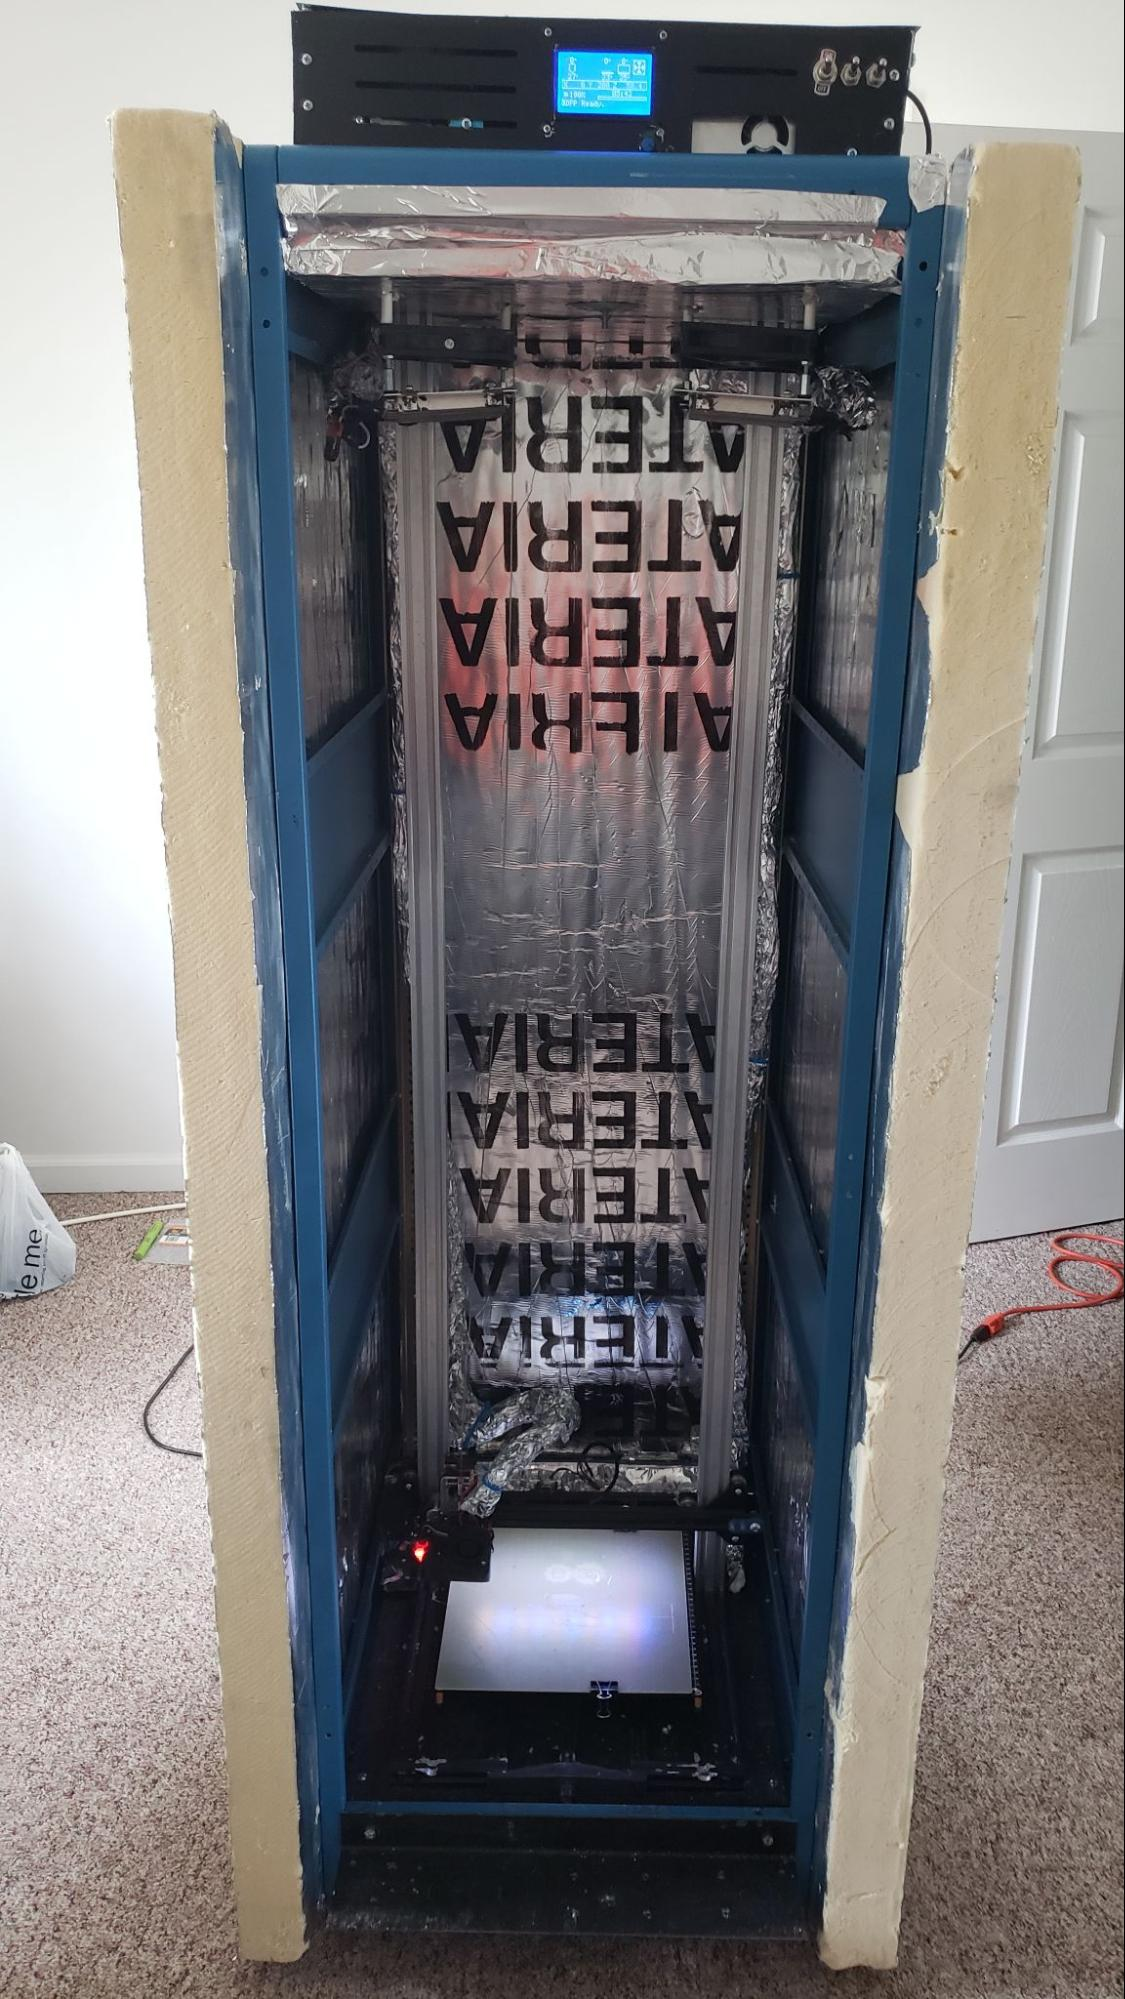
\includegraphics[width=75pt]{printer} %Z how large image is
\end{wrapfigure}

\vspace*{-10pt} % move title's anchor box up closer to title
\leavevmode\subsection{\href{https://github.com/jfcbooth/3dpp}{3D PEEK Printer \scriptsize\faLink}}

Designed and built a large-scale 3D printer capable of printing engineering-grade plastics.
This printer was specialized to print static mixers out of PEEK for biofuel refinement.
Involved in the development was designing the kinematic system, thermal dynamics, and software to safely control it's operation
while dealing with hazardous temperatures and voltages.

% Entry 3 - image on the left
% The Cold Plate

\setlength\intextsep{20pt} % how far image is down from section title
\begin{wrapfigure}[7]{l}{40pt} % # of narrow lines, right top alignment, image L/R adjustment
	%\hspace*{-20pt} % how close horizontal text can be
    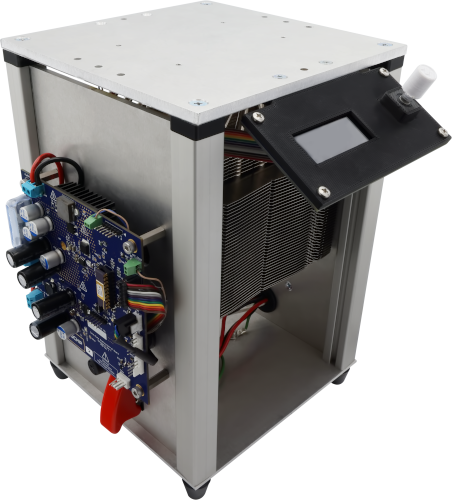
\includegraphics[width=63pt]{cold_plate} %Z how large image is
\end{wrapfigure}

\vspace*{-10pt}
\leavevmode \subsection{\href{https://github.com/microchip-pic-avr-examples/pic16f17146-cold-plate-mplab-mcc}{The Cold Plate \scriptsize\faLink}}
%\vspace*{-5pt} % move image's anchor box up closer to title

A reference design showing the most efficient way to perform common microcontroller tasks on a PIC16
such as temperature measurement, fan control, current monitoring, and UI-control;
all wrapped up into an engaging demo.
It has become Microchip's most copied code repository.

% Entry 4 - image on right
% Hadley Electric Stand

% \setlength\intextsep{7pt} % image in relation to subsection title
% \begin{wrapfigure}[8]{rt}{25pt} % # of narrow lines, right top alignment, image L/R adjustment
% 	\hspace*{-23pt} % how close horizontal text can be
%     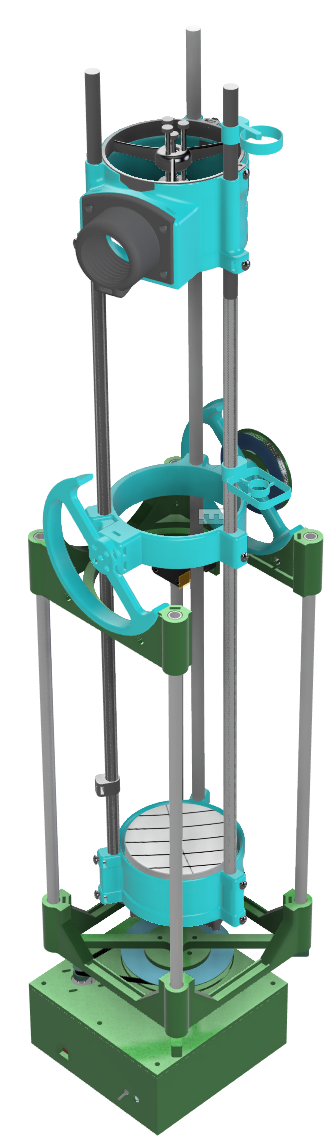
\includegraphics[width=45pt]{hadley_electric_stand2} %Z how large image is
% \end{wrapfigure}

% \vspace*{-10pt} % move title's anchor box up closer to title
% \leavevmode\subsection{\href{https://github.com/jfcbooth/hadley_electric_stand}{Hadley Electric Stand - Open Source Project\scriptsize\faLink}}

% Hadley is a \$150 telescope, capabable of giving 

%----------------------------------------------------------------------------------------
% EDUCATION
\section{Education} 
%----------------------------------------------------------------------------------------



% Each qualification entry is added with a \qualificationentry command. Below is an empty one to use as a template:
%------------------------------------------------

\begin{supertabular}{r l} % Start a table with two columns, the table will ensure everything is aligned

	%------------------------------------------------
	
	\qualificationentry
		{2018-2022} % Duration 
		{Computer Engineering} % Degree
		{Summa Cum Laude; 3.98 GPA; Comp Org SI} % Honors, achievements or distinctions (e.g. first class honors)
		{Bachelors of Science} % Department
		{Shippensburg University of Pennsylvania} % Institution
	
	%------------------------------------------------
	
	\qualificationentry
		{2018-2022} % Duration
		{Mathematics} % Degree
		{} % Honors, achievements or distinctions (e.g. first class honors)
		{Minor} % Department
		{Shippensburg University of Pennsylvania} % Institution
	
	%------------------------------------------------
	

	%------------------------------------------------

\end{supertabular}
% END EDUCATION

%----------------------------------------------------------------------------------------
%	AWARDS
%----------------------------------------------------------------------------------------

\section{Awards}

% This section is laid out using a table. A \tableentry command adds lines with the following parameters:

%\tableentry{Heading}{Content}{spaceafter}
% All 3 parameters must be supplied but any can be empty if you don't need them
% A "spaceafter" value in the third parameter will add some vertical space -- this is to be used between headings, leave it empty for no extra space

%------------------------------------------------

\begin{supertabular}{r l} % Start a table with two columns, the table will ensure everything is aligned
	
	%------------------------------------------------
	
	\tableentry{2020}{Secret Security Clearance (inactive Mar 2022)}{}
	\tableentry{2018}{Eagle Scout}{}
	\tableentry{2017}{CompTia A+ Certified}{}
	
	%------------------------------------------------
	
\end{supertabular}

%----------------------------------------------------------------------------------------
%	COMPUTER SKILLS
%----------------------------------------------------------------------------------------

% \section{Misc. Skills} 

% % This section is laid out using a table. A \tableentry command adds lines with the following parameters:

% %\tableentry{Heading}{Content}{spaceafter}
% % All 3 parameters must be supplied but any can be empty if you don't need them
% % A "spaceafter" value in the third parameter will add some vertical space -- this is to be used between headings, leave it empty for no extra space

% %------------------------------------------------

% \begin{supertabular}{r l} % Start a table with two columns, the table will ensure everything is aligned
	
% 	%------------------------------------------------
	
% 	\tableentry{Beginner}{Java, MS DOS}{spaceafter}
	
% 	%------------------------------------------------
	
% 	\tableentry{Intermediate}{Javascript, Python, HTML, CSS,}{}
% 	\tableentry{}{Microsoft Windows}{}
% 	\tableentry{}{Computer Hardware \& Support}{spaceafter}
	
% 	%------------------------------------------------
	
% 	\tableentry{Expert}{Perl, Unix, \LaTeX}{spaceafter}
	
% 	%------------------------------------------------
	
% \end{supertabular}

%----------------------------------------------------------------------------------------
%	COMMUNICATION SKILLS
%----------------------------------------------------------------------------------------

% \section{Communication Skills}

% % This section is laid out using a table. A \tableentry command adds lines with the following parameters:

% %\tableentry{Heading}{Content}{spaceafter}
% % All 3 parameters must be supplied but any can be empty if you don't need them
% % A "spaceafter" value in the third parameter will add some vertical space -- this is to be used between headings, leave it empty for no extra space

% %------------------------------------------------

% \begin{supertabular}{r l} % Start a table with two columns, the table will ensure everything is aligned
	
% 	%------------------------------------------------
	
% 	\tableentry{Conferences}{Oral Presentation at the Annual MIT}{}
% 	\tableentry{}{Theoretical Physics Conference -- 1987}{spaceafter}
	
% 	%------------------------------------------------
	
% 	\tableentry{Posters}{Poster at the Meeting of the American}{}
% 	\tableentry{}{Physical Society -- 1985}{spaceafter}
	
% 	%------------------------------------------------
	
% \end{supertabular}

%----------------------------------------------------------------------------------------

\end{paracol} % End two-column mode

\section{Core Competancies}
\begin{itemize}
	\itemsep 0pt
	\item \textbf{Technical:} C, Python, Linux, Marlin, Embedded Development, Digital Circuit Design, 3D CAD Design, Data Analytics
	\item \textbf{Software:} Git, Fusion 360, KiCAD, Eagle, Sourcetree, MPLAB X, XC8, Bash, FreeCAD
	\item \textbf{Other:} System Administration, Embedded Communications Protocols (I2C, SPI, DMX, UART, CAN), IT Professional
\end{itemize}
%----------------------------------------------------------------------------------------

\end{document}
